\section{Proposed Solution}
We propose a solution which can convert a Java class file to a UPPAAL SMC model, rewrite it to insert fault injection attack countermeasures and recommend one of these countermeasures. The point of the conversion to a model, is to be able to provide guarantees about certain properties of the program. This makes sense when the Java class file is rewritten and countermeasures are inserted, since it is then possible to guarantee that the program has not become less secure with respect to certain properties.\\

The workflow stages of the solution are illustrated in \cref{fig:workflow}. The stages are labelled with numbers 1-5. Their purposes are detailed in the following.

% burde vi ogs� give mulighed i programmet for bare at f� en ``vanilla'' SMC model ud?

\paragraph{Stage 1 - 2} rewrites the original Java class file to include fault injection countermeasures. The output is one or more modified Java class files depending on the number of countermeasures implemented. 
\paragraph{Stage 2 - 3} provides two options, either one can use the rewritten code to perform static analysis with an analysis tool, or one can parse the code through the solution's parser and generate a UPPAAL SMC model. 
\paragraph{Stage 3 - 4} modifies the model to include a special fault injection template, which can simulate a fault being injected in the Java program. At this point in the workflow, the model of the rewritten code is also modified to include special synchronisations, guards, updates and locations. These make it possible to verify timed properties of the model and enables the fault template to interact with the model.
\paragraph{Stage 3,4 - 5} is where the solution recommends a fitting countermeasure for the code, based properties it has verified about the rewritten version(s) of the code. These models serve as the input for stage 5. The recommended countermeasure incurs the least static size overhead of the rewritten Java class file but provides the most protection for the largest possible duration of the program's execution.

\begin{figure}[H]
\centering
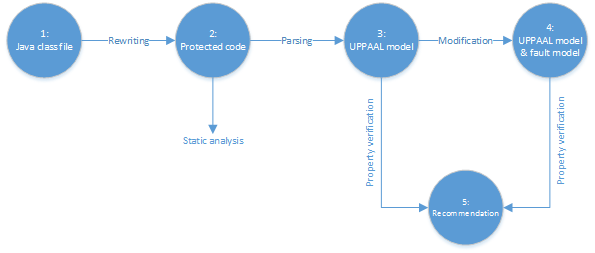
\includegraphics{figures/workflow.png}
\caption{The workflow of the solution, from Java class file to UPPAAL SMC model}
\label{fig:workflow}
\end{figure}
\ch{make better figure}